\documentclass[11pt,]{article}
\usepackage[left=1in,top=1in,right=1in,bottom=1in]{geometry}
\newcommand*{\authorfont}{\fontfamily{phv}\selectfont}
\usepackage{lmodern}


  \usepackage[T1]{fontenc}
  \usepackage[utf8]{inputenc}



\usepackage{abstract}
\renewcommand{\abstractname}{}    % clear the title
\renewcommand{\absnamepos}{empty} % originally center

\renewenvironment{abstract}
 {{%
    \setlength{\leftmargin}{0mm}
    \setlength{\rightmargin}{\leftmargin}%
  }%
  \relax}
 {\endlist}

\makeatletter
\def\@maketitle{%
  \newpage
%  \null
%  \vskip 2em%
%  \begin{center}%
  \let \footnote \thanks
    {\fontsize{18}{20}\selectfont\raggedright  \setlength{\parindent}{0pt} \@title \par}%
}
%\fi
\makeatother




\setcounter{secnumdepth}{0}


\usepackage{graphicx,grffile}
\makeatletter
\def\maxwidth{\ifdim\Gin@nat@width>\linewidth\linewidth\else\Gin@nat@width\fi}
\def\maxheight{\ifdim\Gin@nat@height>\textheight\textheight\else\Gin@nat@height\fi}
\makeatother
% Scale images if necessary, so that they will not overflow the page
% margins by default, and it is still possible to overwrite the defaults
% using explicit options in \includegraphics[width, height, ...]{}
\setkeys{Gin}{width=\maxwidth,height=\maxheight,keepaspectratio}

\title{Repression Strategies and Mass Mobilization }



\author{\Large Yufan Yang\vspace{0.05in} \newline\normalsize\emph{University of Iowa}  }


\date{}

\usepackage{titlesec}

\titleformat*{\section}{\normalsize\bfseries}
\titleformat*{\subsection}{\normalsize\itshape}
\titleformat*{\subsubsection}{\normalsize\itshape}
\titleformat*{\paragraph}{\normalsize\itshape}
\titleformat*{\subparagraph}{\normalsize\itshape}

\newcommand{\dummy}[1]{#1}

\usepackage{natbib}
\bibpunct{(}{)}{;}{a}{}{,}
\bibliographystyle{apsr}
%\usepackage[strings]{underscore} % protect underscores in most circumstances



\newtheorem{hypothesis}{Hypothesis}
\usepackage{setspace}

\makeatletter
\@ifpackageloaded{hyperref}{}{%
\ifxetex
  \PassOptionsToPackage{hyphens}{url}\usepackage[setpagesize=false, % page size defined by xetex
              unicode=false, % unicode breaks when used with xetex
              xetex]{hyperref}
\else
  \PassOptionsToPackage{hyphens}{url}\usepackage[unicode=true]{hyperref}
\fi
}

\@ifpackageloaded{color}{
    \PassOptionsToPackage{usenames,dvipsnames}{color}
}{%
    \usepackage[usenames,dvipsnames]{color}
}
\makeatother
\hypersetup{breaklinks=true,
%            bookmarks=true,
            pdfauthor={Yufan Yang (University of Iowa)},
             pdfkeywords = {repression, mobilization},  
            pdftitle={Repression Strategies and Mass Mobilization},
            colorlinks=true,
            citecolor=black,
            urlcolor=blue,
            linkcolor=black,
            pdfborder={0 0 0}}
\urlstyle{same}  % don't use monospace font for urls

% set default figure placement to htbp
\makeatletter
\def\fps@figure{htbp}
\makeatother



% add tightlist ----------
\providecommand{\tightlist}{%
\setlength{\itemsep}{0pt}\setlength{\parskip}{0pt}}

\begin{document}
	
% \pagenumbering{arabic}% resets `page` counter to 1 
%
% \maketitle

{% \usefont{T1}{pnc}{m}{n}
\setlength{\parindent}{0pt}
\thispagestyle{plain}
{\fontsize{18}{20}\selectfont\raggedright 
\maketitle  % title \par  

}

{
   \vskip 13.5pt\relax \normalsize\fontsize{11}{12} 
\textbf{\authorfont Yufan Yang} \hskip 15pt \emph{\small University of Iowa}   

}

}








\begin{abstract}

    \hbox{\vrule height .2pt width 39.14pc}

    \vskip 8.5pt % \small 

\noindent Previous studies have provided competing theories and mixed empirical
evidence on how repression effects mass mobilization. I argue that the
answer to this question lies in different repression strategies.
Especially, physical rights regression such as political killing,
imprisonment without a legal process, and torture, impairs regime
legitimacy and provides willingness for the public to participate in
collective action. It also provides opportunities for dissent groups to
expand. Hence, physical rights repression tends to escalate mass
mobilization instead of deterring it. In contrast, censorship, which is
the block of information, can isolate the country from the outside
world, isolate the dissent group from the public, and protect the
government's credibility. Therefore, censorship lowers the willingness
for the public to mobilize and reduces the opportunities for dissent
groups to expand. Hence, censorship can successfully deter mobilization.


\vskip 8.5pt \noindent \emph{Keywords}: repression, mobilization \par

    \hbox{\vrule height .2pt width 39.14pc}



\end{abstract}


\vskip 6.5pt


\noindent \doublespacing \section{Introduction}

The interaction between repression and mobilization is a long-standing
debate. Political scientists have agreed that mass mobilization leads to
higher repression, but there is still no consensus on whether repression
successfully deters or escalates mass mobilization. Studies of how
effective state repression is have provided competing theories and mixed
evidence. Different arguments include: an inverted-U relationship
between state repression and conflict (\citet{Muller1990}), a positive
impact that repression escalates conflict (\citet{MasonandKrane1989},
\citet{Goodwin2001}, \citet{Hultquist2017}), and a negative impact that
repression deters or defeats conflict (\citet{Downes2008},
\citet{Lyall2009}). Further, some studies explore the dynamics between
repression and mobilization by looking at different levels or different
types of repression. For example, \citet{Lichbach1987} builds a rational
actor model and finds that low-level repression tends to deter violent
collective action when fear replaces anger. However, \citet{Gupta1993}
argue that high-level repression can also be effective in autocracies.
Nonetheless, \citet{Moore1998}'s empirical evidence supports
\citet{Lichback1987}'s theory instead of \citet{Gupta1993}'s. Later,
\citet{Carey2006} claims that \citet{Moore1998}'s analysis is flawed
because he did not take account of time and argues that repression is
always ineffective in democracies.

In fact, the answer to this question may lie in different types of
repression, as some scholars have noticed, that violent and non-violent
repression probably has distinct impact on mobilization behaviors.
Violent repression refers to physical torture, killing, disappearing,
etc., while non-violent repression usually defined as constraints on
civil rights, especially civil rights of mobilization. Nonetheless, the
development of technology, especially computer science, provides another
strong tool for the government to repress: censorship. Censorship, as an
effective way to block information, widely exists in autocracies. The
public can only receive the information that the state allows them to
receive, contributing to regime legitimacy and social stability. For
instance, one of the reasons that repression escalates mass mobilization
is that, state violence can damage regime legitimacy, so that the
willingness for the public to initiate anti-government collective action
as well as the opportunities for dissent groups to expand increase
\citet{Greene1974}. However, if the state successfully hides the
information on state violence, the public would not have willingness for
mass mobilization. Further, civil rights as a western, democratic term,
can also be manipulated by state censorship in autocracies, making the
public accept the state's ideology and lowering the willingness for
collective action. That is to say, a combination of conventional
repression and censorship can be an effective way to deter mass
mobilization.

Therefore, it is necessary to distinguish these three types of
repression and explore the dynamics between each one and mass
mobilization. This paper builds a model using differential equations to
identify the dynamic interactions within a system of physical rights
repression, civil rights repression, censorship, and mass mobilization.
This paper applies a dynamic model using differential equations to
explore how repression and mass mobilization interact with each other.
More specifically, this paper categories repression strategies into
three categorizes: physical rights repression, civil rights repression,
and censorship. This paper finds that, if a state mostly relies on
violent repression, mass mobilization tends to escalate, which is a
backfire effect. However, when the state is aware of the growth of mass
mobilization, it will intensify censorship to isolate the dissent group.
With intensified censorship and increased violent repression, mass
mobilization can be successfully deterred. Further, if a state has a
high level of censorship at the beginning, the level of mobilization
tends to be stable in the short term, which is unlikely to be a threat
to state authority. After a certain time, mass mobilization can still
slightly increase, but physical rights repression and censorship will
grow correspondingly. After censorship and physical rights repression
reaches the peak, mass mobilization can be successfully deterred as
well.

\vspace{3mm}

\section{Repressive Strategies and Mass Mobilization}

States have various tools of repression. On the one hand, the state can
use violence to directly eliminate the dissents' capability of
mobilization. These tools include: killings by the government without
due process of law; making people disappeared out of political reasons;
incarcerating citizens out of political reasons; and tortures of
individuals from the government. These tools are aimed to make dissents
physically unable to make any collective action, and they are
categorized as physical rights repression in this paper.

On the other hand, the state can limit the dissents' capability of
mobilization in two ways. First, the state can constraint civil rights
such as freedom of movement, freedom of religion, freedom of ideology,
etc., which reduces the opportunities of mass mobilization. These tools
are categorized as civil rights repression in this paper. Second, with
the help of technology, the state can simply block information that
threatens regime legitimacy or state authority. This information can be
news that reveals states' violation of human rights, news that reveals
government officials such as corruption, as well as ideologies of
democracy, liberty, human rights, and so on. Blocking threatening
information can lower the public's willingness of mobilization, and thus
is widely applied in autocracies. Physical rights repression, civil
rights repression, and censorship can have different even opposite
impact on mobilization, and this is why previous studies have presented
distinct empirical results.

\section{Physical Rights Repression}

Physical rights repression is violent. It might be the most effective
way to stop individuals from joining collective action, but it tends to
be counterproductive overall. For one thing, state violence against
civilians impairs the regime legitimacy and provides more willingness
for the dissent group and the public to escalate mass mobilization
(\citet{Goodwin2001}). For another, state violence, especially
indiscriminate violence against civilians, may even convince the public
who are previously inactive to join the dissent group to seek for
protection and survival (\citet{Kalyvas2007}). In short, physical rights
repression increases willingness for the dissents and general public of
collective action, as well as opportunities for the dissents to expand
their influence. Therefore, physical rights repression alone is at best
ineffective and at worst counterproductive (\citet{Kalyvas2006}).

\textit{Hypothesis 1: Physical rights repression escalates mass mobilization.}

\section{Civil Rights Repression}

Civil rights repression can be complicated. To reduce the dissents'
capability of mobilization without using violence, the state tends to
constrain freedom of peaceful assembly, freedom of religion, freedom of
speech, and freedom of movement. These tools are usually pre-emptive and
can be effective if the state use these tools constantly. Though the
violation of these human rights can lead to social frustration and
anger, constant repression on civil rights can keep the opportunities of
mass mobilization at a low level. Nonetheless, constant repression on
civil rights requires considerable investment and detailed
implementation strategies, such as governmental spending on police and
secret police in order to monitor and control civilians. Governmental
investment on civil rights repression can fluctuate over time, and given
this inconsistency, it is hard to tell whether civil rights repression
can effectively deter mass mobilization in reality.

\section{Censorship}

Hiding, blocking, and manipulating information is the subtlest way of
repression, and sometimes the public are not even aware of this type of
repression since the information is not available. As previously
mentioned, two types of information are the most likely to be censored:
negative information on the government and information of democracy,
liberty, human rights, and collective action (\citet{King2013}).
Censorship tends to be the most effective repression strategy for the
following reasons. First, censorship isolates the country from the
outside world, and thereby democratic values are not easily to be passed
on to citizens in authoritarian regimes. Even if the public is aware of
democratic values, it is unlikely that they are fully convinced by them,
which happens in China (\citet{LuandShi2015}), because the state has the
power to decide what kind of information its citizens can receive.
Therefore, the willingness of the public to start anti-regime
mobilization towards autocracies is low. Second, censorship helps to
hide negative news about the government and government officials. The
state may censor the information that would damage the image,
reputation, or credibility of governments, so that social frustration
and anger is low. In this case, the public simply has no reason to join
collective action. This type of censorship can happen in both
autocracies and democracies. Finally, censorship isolates dissent
groups. If the dissent group wants to expand by seeking for new members,
signals have to be delivered to the public. However, censorship can
successfully cut off the channel whereby dissents speak to the public.
Further, when the state uses selective repression on the dissent group,
such as killings and imprisonment, which can impair regime legitimacy,
censorship lowers the damage by not letting the public know about the
state's violation of human rights. Hence, the possibility of the
aforementioned backfire effect is low.

\textit{Hypothesis 2: Information repression (censorship) deters mass mobilization.}

\vspace{3mm}

\section{Research Design}

In this research, the unit of analysis is country-year, and the data
cover 162 countries between 1990 and 2016. The dependent variables are
\textit{the number of total protest} and
\textit{the numbers of violent protest}, from \citet{ClarkandRegan2016}.
There are four independent variables of repression:
\textit{physical rights repression}, \textit{civil society repression},
\textit{government’s effort on media censorship}, and
\textit{government’s effort on internet censorship}. The first two
variables are from CIRI Human Rights project, and the last two variables
are from V-Dem version 9. Originally, all these four variables are coded
in a way of measuring government's respect for these human rights, that
higher values indicate lower repression. To make the results more
intuitive, I recoded these four variables reversely, that higher values
indicate higher repression. Control variables include:
\textit{GDP per capita (logged)}, \textit{total population (logged)},
and \textit{democracy index}. The first two variables are from World
Bank, and the variable of democracy is from V-Dem version 9.

\section{Description of Protest}

Graph 1 and Graph 2 show the numbers of total protest and violent
protest in the world over time. Both graphs present that, though the
number of protest fluctuates over time, the recent decade has witnessed
a sharp growth of mass mobilization after 2010. Graph 3 and Graph 4 show
the numbers of total protest and violent protest by region. Overall,
Middle East has the lowest level of total protest and violent protest,
Africa and Europe have higher standard deviation compared with other
regions.

\begin{center}
    \textbf{Graph1}
\end{center}

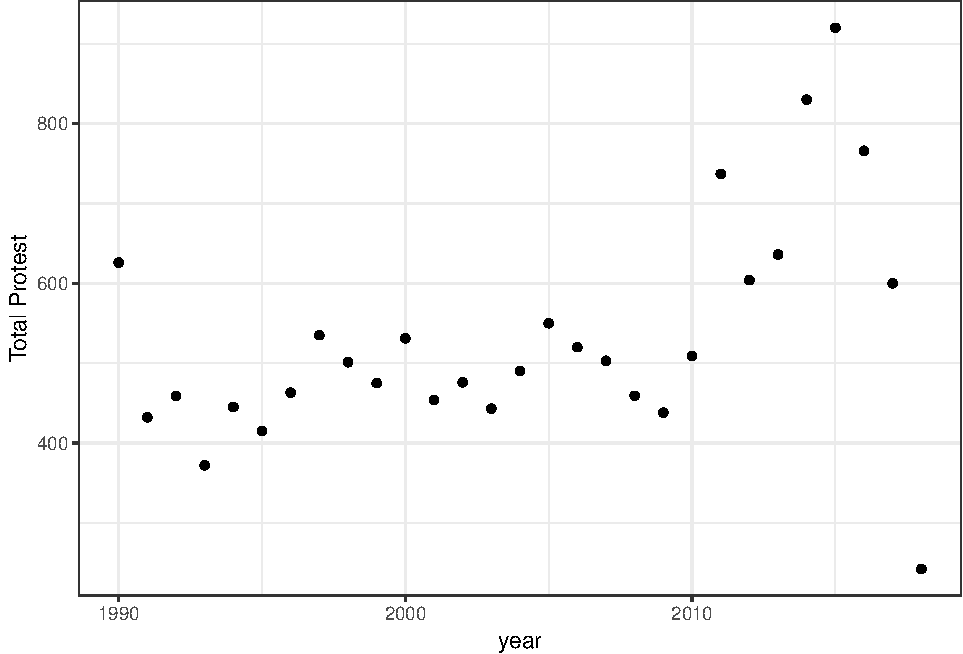
\includegraphics{replication_files/figure-latex/unnamed-chunk-2-1.pdf}

\begin{center}
    \textbf{Graph2}
\end{center}

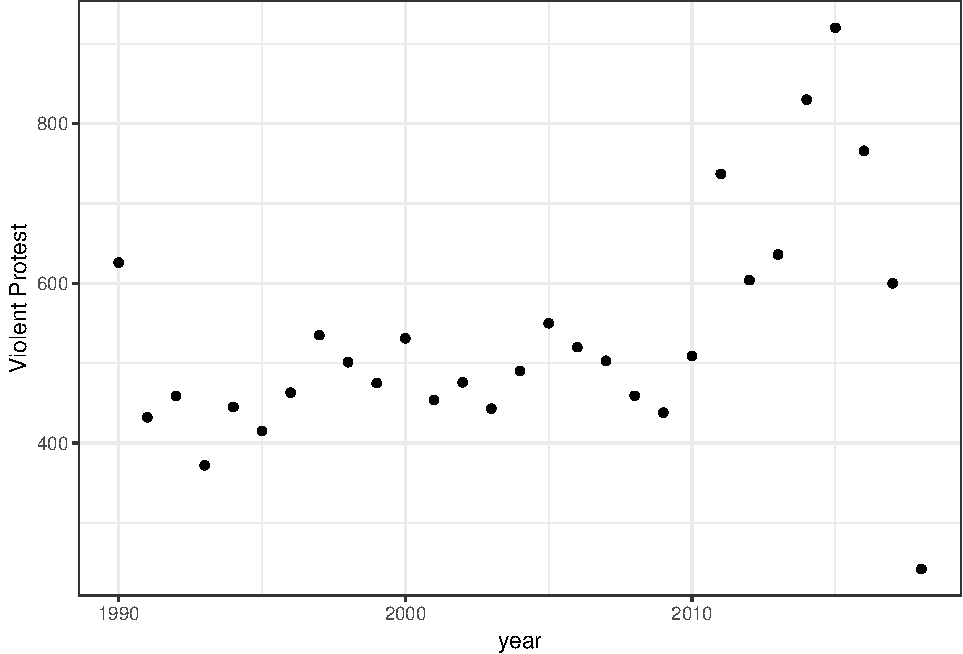
\includegraphics{replication_files/figure-latex/unnamed-chunk-3-1.pdf}

\begin{center}
    \textbf{Graph3}
\end{center}

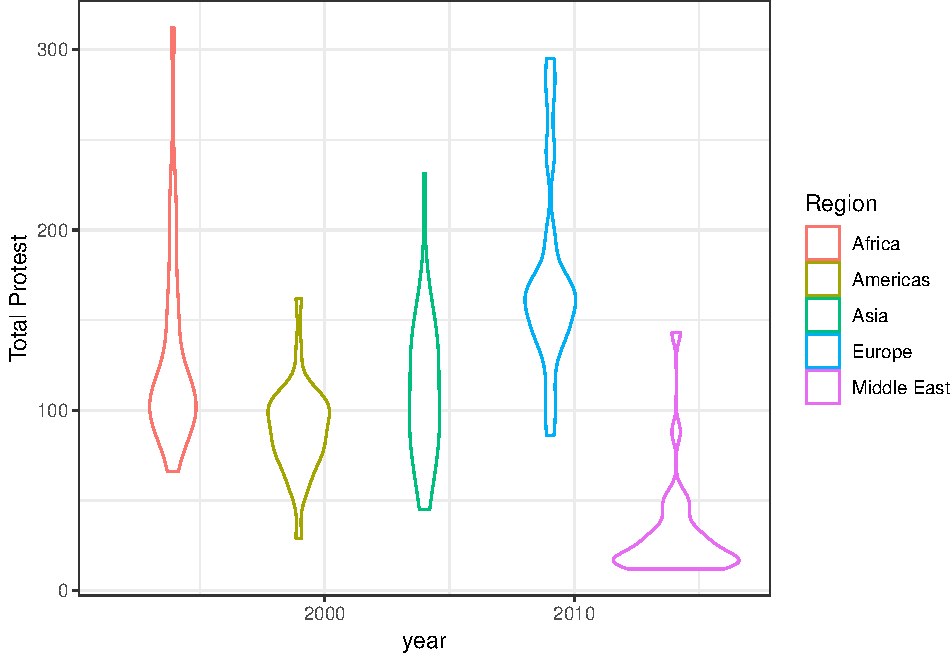
\includegraphics{replication_files/figure-latex/unnamed-chunk-4-1.pdf}

\begin{center}
    \textbf{Graph4}
\end{center}

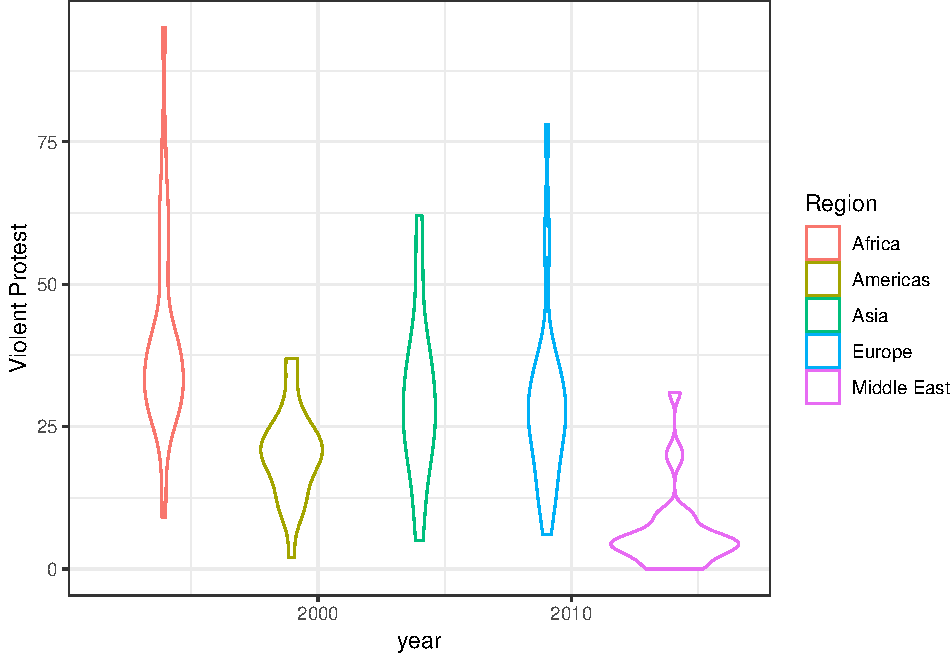
\includegraphics{replication_files/figure-latex/unnamed-chunk-5-1.pdf}

\section{Empirical Evidence}

I run a panel regression model with random effects to see how different
repression strategies shape collective action behavior. The results are
shown in Graph 5 and Graph 6. The dependent variable in Graph 5 is
\textit{total protest}. The orange line is the baseline model, in where
only four independent variables of repression strategies are included.
The blue line represents the full model, where all control variables are
included and region is controlled for. Graph 5 shows that
\textit{physical rights repression} is positively correlated with
\textit{total protest} while \textit{media censorship} is negatively
correlated with \textit{total protest}, and these two results are
significant in both models. That is to say, physical rights repression
tends to escalate mass mobilization, while media censorship can
effectively deter it. Graph 6 is similar, except that the dependent
variable is \textit{violent protest}. Likewise, physical rights
repression escalates violent mass mobilization, and media censorship
deters it. Both hypothesis 1 and hypothesis 2 are confirmed. Another
thing to be noticed is that, civil rights repression shows insignificant
results in three out of four models. It is only significant when the
dependent variable is violent protest and other control variables are
added in. This result indicates that the impact of civil rights
repression is not robust, that it can deter mobilization in some
situation, but stays ineffective in some other situation.

\begin{center}
    \textbf{Graph5}
\end{center}

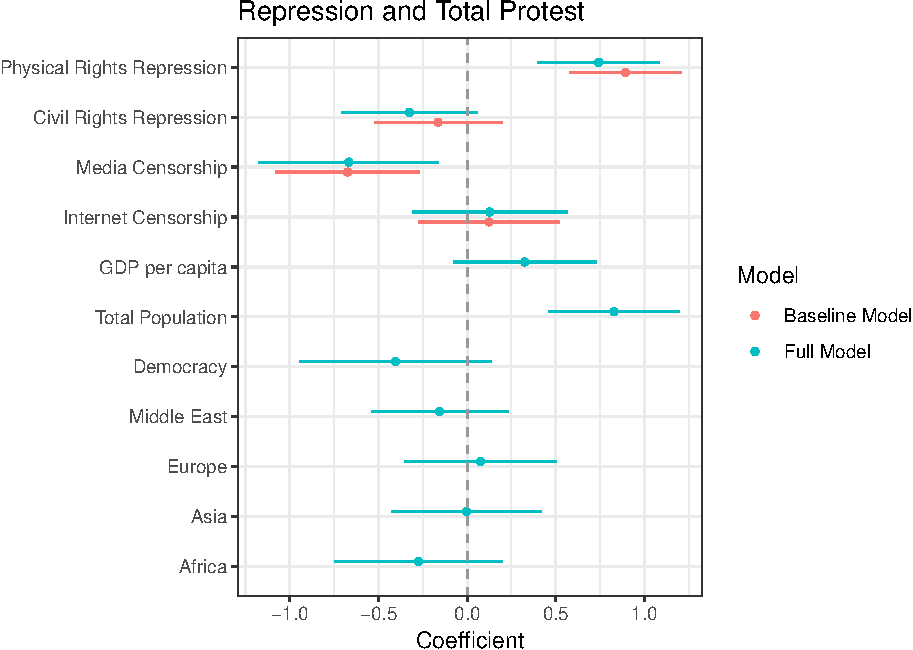
\includegraphics{replication_files/figure-latex/unnamed-chunk-7-1.pdf}

\begin{center}
    \textbf{Graph6}
\end{center}

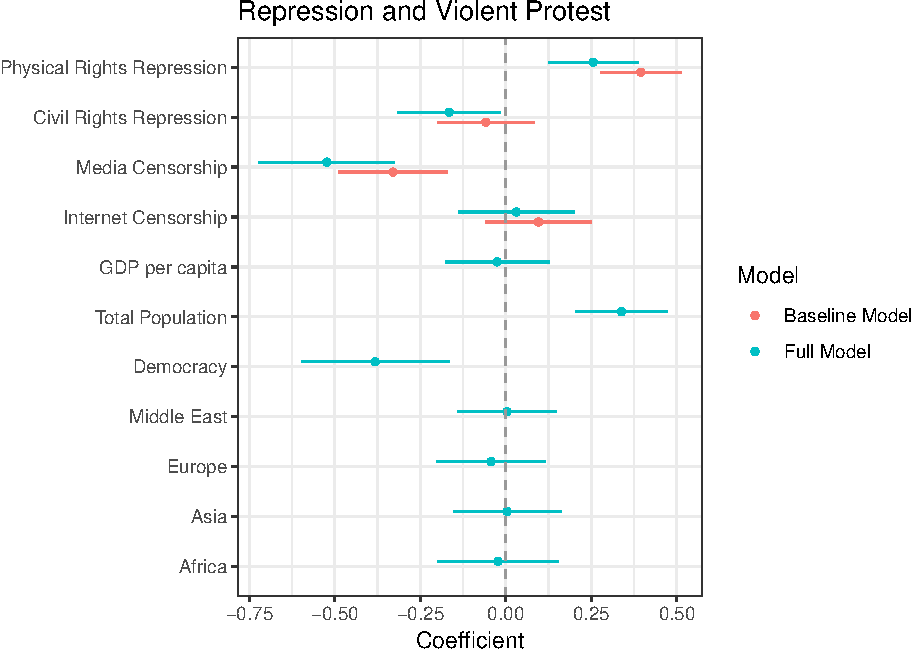
\includegraphics{replication_files/figure-latex/unnamed-chunk-8-1.pdf}

\section{Conclusion}

Previous studies have provided competing theories and mixed empirical
evidence on how repression effects mass mobilization. This paper shows
that, the answer to this question lies in different repression
strategies. Physical rights repression, such as killing, imprisonment,
and torture, can damage regime legitimacy and even motivates the public
to join dissent groups. Hence, physical rights repression tends to have
a backfire effect that it escalates mass mobilization. In contrast,
censorship can effectively deter mass mobilization by isolating the
country from outside world, isolating the dissent group from the public,
and eliminating negative news on government. Thus, censorship lowers the
willingness for the public to take part in collective action and also
reduces the opportunities for the dissent group to expand. Hence,
censorship is in fact the most effective repression strategy.

\section{Appendix}

\begin{table}[!htbp] \centering 
  \caption{Panel Regression with Random Effect} 
  \label{} 
\begin{tabular}{@{\extracolsep{5pt}}lcccc} 
\\[-1.8ex]\hline 
\hline \\[-1.8ex] 
 & \multicolumn{4}{c}{\textit{Dependent variable:}} \\ 
\cline{2-5} 
\\[-1.8ex] & \multicolumn{2}{c}{Total Protest} & \multicolumn{2}{c}{Violent Protest} \\ 
\\[-1.8ex] & (1) & (2) & (3) & (4)\\ 
\hline \\[-1.8ex] 
 Physical Rights Repression & 0.360$^{***}$ & 0.298$^{***}$ & 0.149$^{***}$ & 0.096$^{***}$ \\ 
  & (0.065) & (0.070) & (0.023) & (0.025) \\ 
  & & & & \\ 
 Civil Rights Repression & $-$0.058 & $-$0.113$^{*}$ & $-$0.019 & $-$0.053$^{**}$ \\ 
  & (0.065) & (0.068) & (0.023) & (0.025) \\ 
  & & & & \\ 
 Media Censorship & $-$0.528$^{***}$ & $-$0.514$^{**}$ & $-$0.229$^{***}$ & $-$0.359$^{***}$ \\ 
  & (0.162) & (0.199) & (0.056) & (0.070) \\ 
  & & & & \\ 
 Internet Censorship & 0.104 & 0.106 & 0.071 & 0.023 \\ 
  & (0.172) & (0.185) & (0.058) & (0.063) \\ 
  & & & & \\ 
 GDP per capita &  & 0.293 &  & $-$0.019 \\ 
  &  & (0.186) &  & (0.060) \\ 
  & & & & \\ 
 Total Population &  & 0.684$^{***}$ &  & 0.241$^{***}$ \\ 
  &  & (0.156) &  & (0.049) \\ 
  & & & & \\ 
 Democracy &  & $-$1.867 &  & $-$1.556$^{***}$ \\ 
  &  & (1.281) &  & (0.449) \\ 
  & & & & \\ 
 Europe &  & 0.252 &  & $-$0.118 \\ 
  &  & (0.721) &  & (0.223) \\ 
  & & & & \\ 
 Middle East &  & $-$0.830 &  & 0.017 \\ 
  &  & (1.053) &  & (0.330) \\ 
  & & & & \\ 
 Asia &  & $-$0.014 &  & 0.012 \\ 
  &  & (0.814) &  & (0.253) \\ 
  & & & & \\ 
 Africa &  & $-$0.835 &  & $-$0.058 \\ 
  &  & (0.735) &  & (0.229) \\ 
  & & & & \\ 
 Constant & 1.934$^{***}$ & $-$9.804$^{***}$ & 0.196 & $-$2.473$^{***}$ \\ 
  & (0.415) & (2.907) & (0.142) & (0.914) \\ 
  & & & & \\ 
\hline \\[-1.8ex] 
Observations & 2,628 & 2,580 & 2,628 & 2,580 \\ 
R$^{2}$ & 0.013 & 0.026 & 0.019 & 0.035 \\ 
Adjusted R$^{2}$ & 0.012 & 0.022 & 0.018 & 0.031 \\ 
F Statistic & 35.406$^{***}$ & 69.547$^{***}$ & 51.966$^{***}$ & 92.826$^{***}$ \\ 
\hline 
\hline \\[-1.8ex] 
\textit{Note:}  & \multicolumn{4}{r}{$^{*}$p$<$0.1; $^{**}$p$<$0.05; $^{***}$p$<$0.01} \\ 
\end{tabular} 
\end{table}




\newpage
\singlespacing 
\bibliography{references.bib}

\end{document}